\section{mSTS assembly and its services}

 The silicon detector comprises $11$ modules ($22$ \glspl{FEB}) and $2$ pulser boards. Each module consists of a silicon sensor, shielded microcables, and $2$ \glspl{FEB}. Two different silicon sensor sizes were used to assemble \gls{mSTS} modules - $62\times62$\,mm and $62\times124$\,mm. Each side of the sensor has $1024$ strips which are connected via microcables to the readout electronics - $8$ STS-XYTERs on the \gls{FEB}. The low-mass microcables transport the analog signals, and they can be affected by any electromagnetic interference~(\gls{EMI}). The analog signals received by the STS-XYTER chips are then amplified and converted into digital hit data words. Subsequently, the digital signals are transported via the data cables to \glspl{CROB} (in total $5$ readout boards - one for each \gls{mSTS} ladder) to the \gls{CRI}, and then from there to the \gls{FLES}, where they are processed and stored for analysis. In total, \gls{mSTS} has $22 528$ readout channels, which constitute only $1.25$\% of the final detector. In order to avoid overheating and reduce noise, the \gls{FEE} needs to be properly cooled and powered.  
\subsection{Powering of the detector modules}
\label{module}
The powering of the \gls{mSTS} is organized similarly as it will be implemented for the final \gls{STS} (see section~\ref{sts_module} and figure~\ref{fig_msts_scheme})~\cite{Koczon:2020Jc}. Each power board (in total $5$ \glspl{POB} - one for each ladder) is populated with DC/DC converters ($1.8$\,V and $2.4$\,V, $2.5$\,V and $3$\,V\,\cite{DC_DC_converter}). These boards are connected to the low voltage power supply (WIENER~\cite{wiener}). The double-sided silicon sensors are symmetrically reverse-biased ($\pm 75$\,V) and operated in a constant voltage mode. Each side of the sensor is connected to a high-voltage module located in the same crate as the low-voltage ones. The details of the powering scheme and the modules mounted on the carbon ladders can be seen in Figure~\ref{fig_msts_scheme}.

\begin{figure}[!h]
\centering
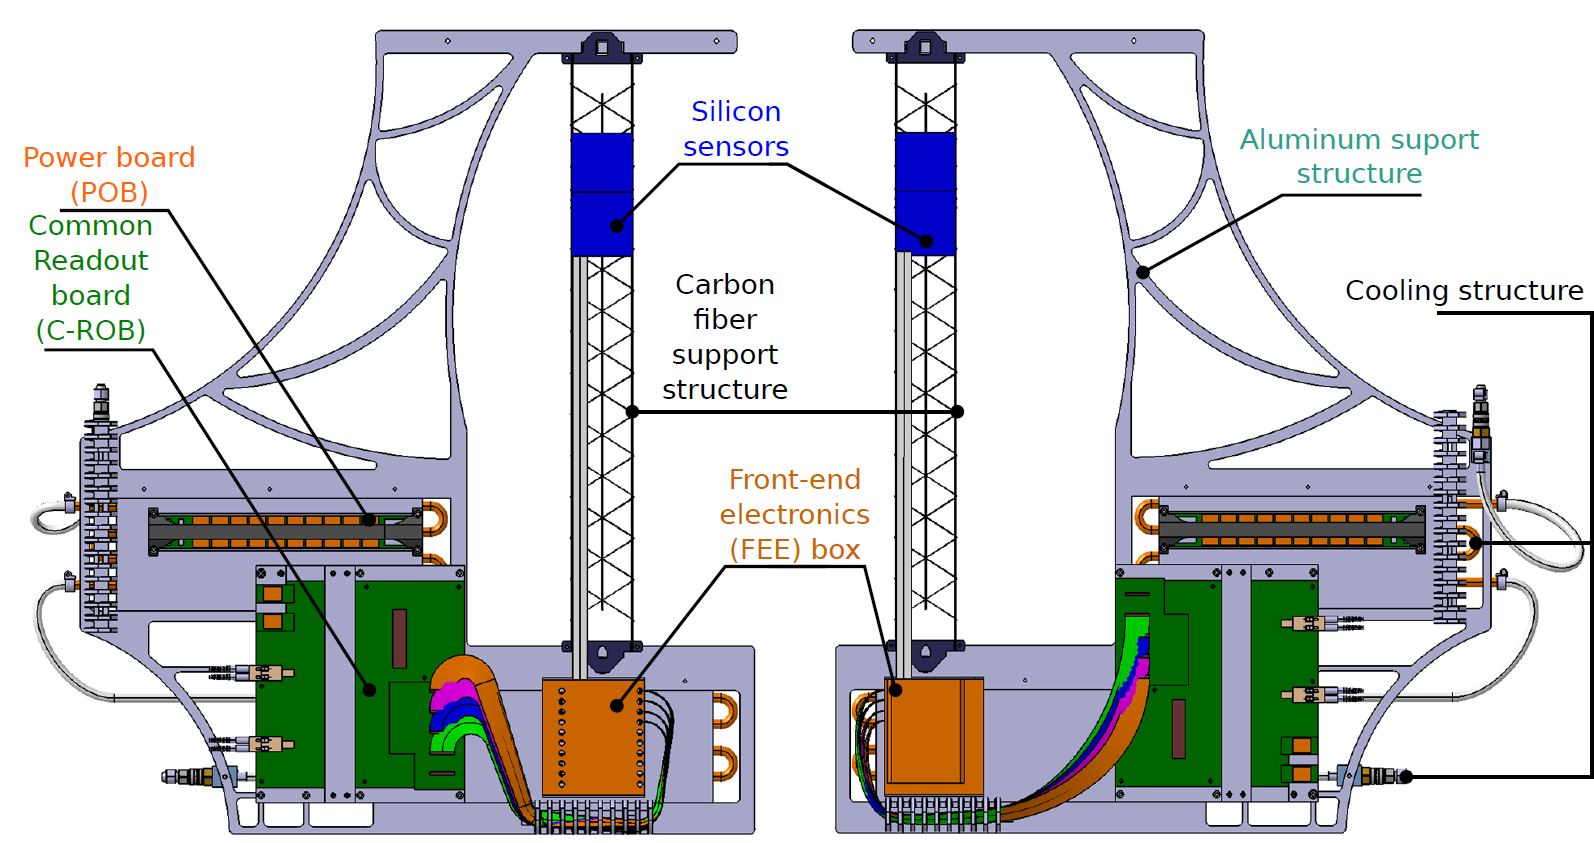
\includegraphics[width=0.9\columnwidth]{Chapter6/DCS/images/unit0.png}
\caption{Schematic view of the first station of the \gls{mSTS}. It depicts the main structures of the C-Frame. }
\label{fig_msts_scheme}
\end{figure}
\newpage


\subsubsection{Noise considerations}
Noise\footnote{Unwanted high-frequency disturbance or interference with outside electrical signals.} problems are the most common and critical issues while building a particle detector. In an environment with many devices, noise sources may be difficult to detect, and it could be sometimes even more difficult to minimize the interference. The total noise contribution can be divided into four components~\cite{noise_twepp2008}:
\begin{itemize}
    \item Thermal noise $n_{TH}(t)$
    \item Electromagnetic interference (\gls{EMI}) between the detector and \gls{FEE} connection, $n_{D-E}(t)$
    \item \gls{EMI} between \gls{FEE} and external connections, $n_{E-F}(t)$
    \item Additional sources, related to the intrinsic noise of the FEE elements, $n_{add}(t)$
\end{itemize}

From the practical point of view, designing and implementing a proper powering and grounding scheme play a critical role in the data quality from the detector~\cite{Bobillier:1159563}. The silicon sensors are characterized by very low signal levels, which makes them particularly sensitive to noise pickup. In the case of the \gls{mSTS}, the \gls{FEE} is located between 45\,cm and $49$\,cm from the silicon sensor. The microcables connecting the two mentioned elements (sensor and \gls{FEB}) are shielded, but the \gls{EMI} of the analog signal could be clearly observed when the cables are not completely flat (due to e.g., external stresses).  The other contribution which is related to the noise picked up between the \gls{FEE} and external connections is suppressed by an additional filter box (first order RC-filter) for the silicon sensor biasing lines. The total noise in the system serves as a reference for the minimum signal level that could be processed. More detailed considerations about the intrinsic noise influence on the system are described in the section~\ref{module}. During the laboratory tests, satisfactory performance of the detector modules was achieved ($1000$~e \gls{ENC}). Nevertheless, the performance in the experiment area can differ greatly, due to the influence of devices belonging to other subsystems or the accelerator services. The problem with the noise performance of the modules was also identified in this case, and substantial efforts were taken in order to find the noise sources and limit their influence (increasing the analog-digital converters (\gls{ADC}) threshold values of the STS-XYTERs). 

The appropriate grounding of the \gls{FEE} reduces capacitive coupling between the structure and the sensitive areas of the \gls{FEE}. Furthermore, it generates low impedance at the power connector input to reduce external current interference going through FEE electronics. The \gls{mSTS} enclosure is connected to a dedicated ground of the \gls{mCBM} experiment, preventing any \gls{EMI} in the lines that may affect the performance. The \gls{mSTS} enclosure is decoupled from the experiment table (no direct connection of any conducting elements). In reality, there are no perfect grounds, even in the same line there might be potential differences. 

Figure~\ref{fig_msts_power} depicts the power distribution of the \gls{mSTS}. The floating ground scheme for the sensors biasing circuity and the front-end electronics come with important boundary conditions for the powering - each module side requires a separate powering line~\cite{RodriguezRodriguez2020}. In order to further reduce possible noise pickup, a return path capacitor was implemented at the \gls{FEB} connectors and the \gls{HV} common return (depicted as C-RTN) was connected to the enclosure.

\begin{figure}[!h]
\centering
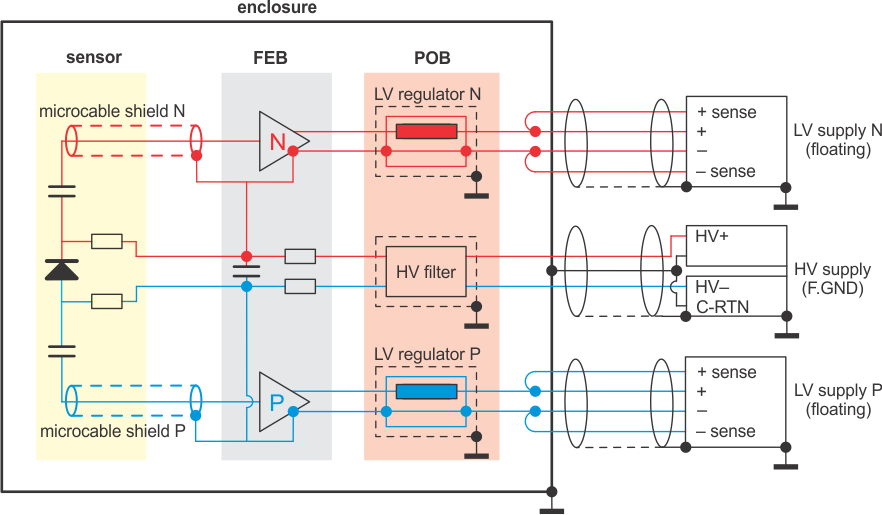
\includegraphics[width=0.95\columnwidth]{Chapter6/DCS/images/power_distribution.png}
\caption{Power distribution scheme of the \gls{mSTS}~\cite{Lymanets}.}
\label{fig_msts_power}
\end{figure}

\subsection{Detector modules}
 The detector modules used to build \gls{mSTS} differ not only in microcable lengths, and sensor size but also in the version of \gls{LDO} regulators and DC/DC converters output voltage, which may affect parameters like power dissipation or the general performance (ENC levels). The module assembly is more broadly discussed in section \ref{module}. The respective components of each \gls{mSTS} unit can be found in Table~\ref{tab:msts_comp}. Before assembling \gls{mSTS}, extensive measurements of all the building blocks were performed. Figure \ref{fig_msts_ENC1} and  \ref{fig_msts_ENC2} show noise measurements of two modules from different units. Unit $1$ is the only unit used before for the previous \gls{mCBM} campaign~\cite{heuser1}. It is one of the oldest units, and it is also slightly irradiated, thus sensors leakage currents are higher than the new modules. The module of unit $1$ (Figure \ref{fig_msts_ENC2}) has larger noise and a more pronounced odd-even effect than unit $0$ module. In both modules, the Z-strips (p-side channel numbers $0$ to $134$) are clearly recognizable. 

Figure \ref{fig_msts_ENC2} also shows the estimated ENC values for different components of the module (sensor, microcables, and \gls{ASIC}s). The \gls{ENC} estimation is based on a simple parameterization of the \gls{ENC} versus capacitance for the STS-XYTER. The targeted \gls{ENC} value for \gls{mSTS} modules is $1000$\,e, but the measurement outcome depends also on the sensor size, microcables length, and nuances of the assembly process. In the case of \gls{mSTS} modules the targeted \gls{ENC} value was achieved during the laboratory testing. Nevertheless, based on the  obtained data and the \gls{ADC} thresholds settings used during the data-taking campaign it was concluded that the \gls{ENC} levels were higher than $1000$\,e.


\begin{table}[!h]
%\caption{mSTS units and differences between the components used for assembly (in order to achieve 1.2\,V output, 1.8\,V \gls{LDO} regulator was used with a diode).}
\caption{Description of the main components of \gls{mSTS} units. During the module assembly, different versions of the components were used. An important difference was the use of SCL $1.8$\,V \gls{LDO} regulators in combination with a diode to achieve the necessary $1.2$\,V operation potential in the \glspl{ASIC}.}
\centering
\resizebox{\textwidth}{!}{%
\begin{tabular}{lllllll}
\hline
Unit & Ladder & Silicon sensors                                                                          & Microcables                                                      & \begin{tabular}[c]{@{}l@{}}DC/DC \\ converters\end{tabular} & \begin{tabular}[c]{@{}l@{}}STS-XYTER\\  version\end{tabular} & \gls{LDO} regulators             \\ \hline
0    & 0      & \begin{tabular}[c]{@{}l@{}}62x62 $\mathrm{mm^{2}}$\\ 62x62 $\mathrm{mm^{2}}$\end{tabular}                  & \begin{tabular}[c]{@{}l@{}}490 mm\\ 450 mm\end{tabular}          & 2.5 V, 3 V                                                  & 2.2                                                          & 1.8\,V and 1.2\,V            \\ \hline
1    & 0      & \begin{tabular}[c]{@{}l@{}}62x62 $\mathrm{mm^{2}}$\\ 62x62 $\mathrm{mm^{2}}$\end{tabular}                  & \begin{tabular}[c]{@{}l@{}}490 mm\\ 450 mm\end{tabular}          & 2.5 V, 3 V                                                  & 2.1                                                          & 1.8\,V and 1.8\,V with diode \\ \hline
2    & 0      & \begin{tabular}[c]{@{}l@{}}62x62 $\mathrm{mm^{2}}$\\ 62x124 $\mathrm{mm^{2}}$\end{tabular}                 & \begin{tabular}[c]{@{}l@{}}490 mm\\ 420 mm\end{tabular}          & 2.5 V, 3 V                                                  & 2.2                                                          & 2.4\,V and 1.2\,V             \\ \hline
3    & 0      & \begin{tabular}[c]{@{}l@{}}62x62 $\mathrm{mm^{2}}$\\ 62x62 $\mathrm{mm^{2}}$\\ 62x62 $\mathrm{mm^{2}}$\end{tabular} & \begin{tabular}[c]{@{}l@{}}490 mm\\ 450 mm\\ 420 mm\end{tabular} & 2.4 V, 2.4 V                                                & 2.1                                                          & 1.8\,V and 1.8\,V with diode \\ \hline
3    & 1      & \begin{tabular}[c]{@{}l@{}}62x124 $\mathrm{mm^{2}}$\\ 62x124 $\mathrm{mm^{2}}$\end{tabular}                & \begin{tabular}[c]{@{}l@{}}490 mm\\ 420 mm\end{tabular}          & 2.4\,V, 2.4 V                                                & 2.1                                                          & 1.8\,V and 1.8\,V with diode \\ \hline
\end{tabular}%
}
\label{tab:msts_comp}
\end{table}
\newpage

\begin{figure}[!hb]
\centering
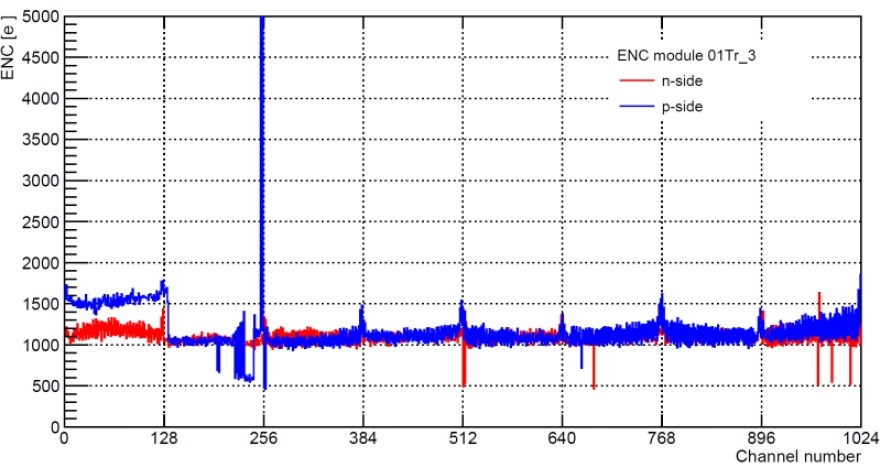
\includegraphics[width=0.9\columnwidth]{Chapter6/DCS/images/U0M1_ENC.jpg}
\caption{Equivalent Noise Charge for module $0$ of unit $0$ measured at the \gls{mCBM} experimental site~\cite{Adrian}. Values from all the analog channels ($128$ per chip) of the \glspl{ASIC} are depicted.}
\label{fig_msts_ENC1}
\end{figure}


\begin{figure}[!h]
\centering
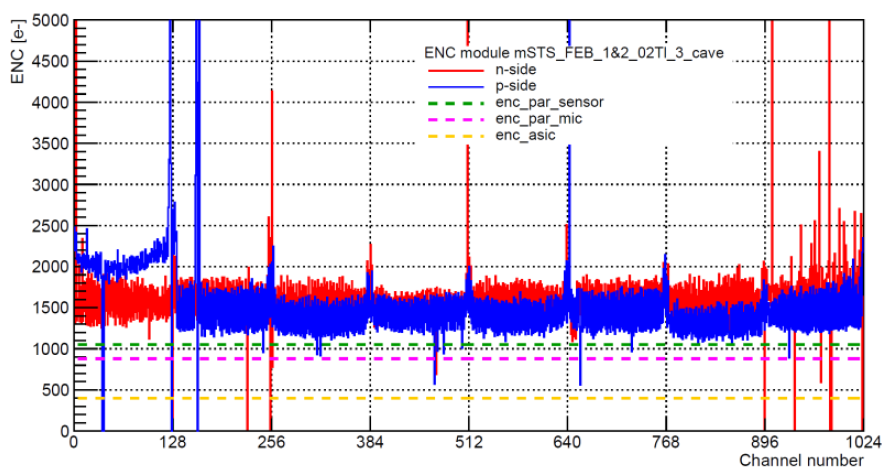
\includegraphics[width=0.9\columnwidth]{Chapter6/DCS/images/U1M1_ENC.png}
\caption{Equivalent Noise Charge plot for module $0$ of unit $1$ measured at the \gls{mCBM} experimental site~\cite{Adrian}. Three additional lines describing the noise contribution from ASIC, ASIC+microcables and ASIC+microcables+sensor are depicted.}
\label{fig_msts_ENC2}
\end{figure}


\subsection{Considerations about the detector cooling}
\label{msts_cooling}
In order to avoid overheating of the \gls{FEE} and \glspl{POB}, the electronics need to be cooled. The cooling system for \gls{mSTS} is a water-based  system, where the main heat exchange elements inside the detector are cooling plates. Three Lauda chillers~\cite{Lauda1} were used to pump chilled water through the cooling plate and efficiently evacuate excess heat. These chillers were also integrated into the control system via RS232-to-Ethernet converter.

Figure~\ref{fig_cooling} depicts the bath temperature\footnote{The temperature of the water inside the chiller is considered a bath temperature.} during the $430$ days of operation. Initially, \gls{mSTS} was cooled with two Lauda chillers. During the data taking in June 2022, one of the chillers failed due to radiation-induced damage (depicted in Figure~\ref{fig_cooling}). Since a similar chiller was unavailable, two others, less powerful units were employed. Hence, the values from the third cooling unit can be seen only during the last months of operation. 

Figure~\ref{fig_cooling} also shows the dew point inside the \gls{mSTS}, which should always be below the coolant temperature, in order to avoid condensation on the \gls{FEE}. The coolant temperature that enters the detector is slightly higher (depending on the actual temperature in the experiment location). This difference ensures that there is no risk related to the condensation inside the detector. The dew point changes are summarized in Figure~\ref{fig_cooling}. It is calculated based on the measured \gls{RH} and temperature, which change depending on the conditions (\gls{FEE} on/off, seasons of the year). In addition to that, the \gls{mSTS} enclosure is not tight,  allowing air circulation.
\begin{figure}[!h]
\centering
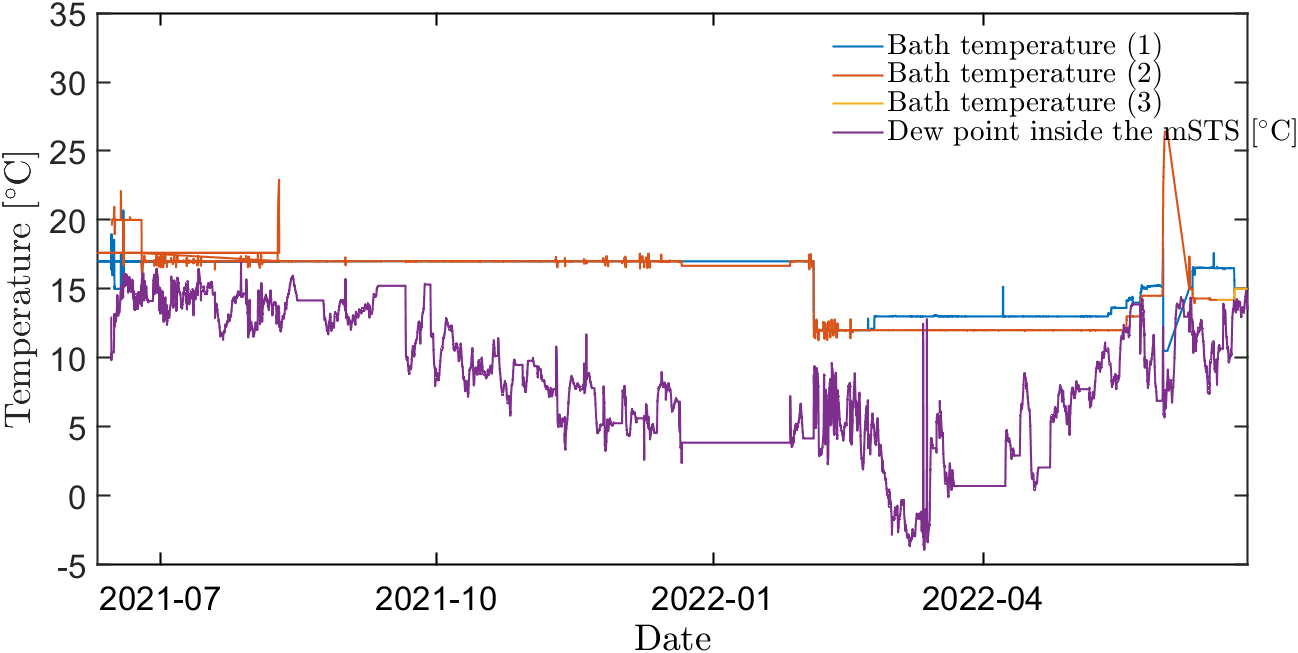
\includegraphics[width=0.95\columnwidth]{Chapter6/DCS/images/cooling.png}
\caption{Temperature readouts of the three Lauda chillers used for the \gls{mSTS} and the dew point inside the enclosure. The period without beam time is shown as a grey area. The red rectangle represents an example of the period when the system was completely off.}
\label{fig_cooling}
\end{figure}

\subsection{Installation of the mSTS detector}
Figure \ref{fig_msts_state} depicts the assembly process of \gls{mSTS}. Before transferring the detector to the \gls{mCBM} experiment, modules of every unit were tested several times (to access the noise related performance by measuring ENC):
\begin{itemize}
    \item Before ladder assembly
    \item After installation on the unit
    \item After assembling the C-frame in the mSTS enclosure
\end{itemize}
The detector services (\gls{LV}, \gls{HV}, cooling), as well as the optical fiber panel were installed on the \gls{mSTS} enclosure front wall~\cite{tekli1}. At that point, the detector was ready to be transferred to the experimental area and the commissioning began.

\begin{figure}[h!]
\centering
\includegraphics[width=0.99\columnwidth]{Chapter6/DCS/images/msts_all.png}
\caption{Assembly process of the \gls{mSTS} (from left to right).}
\label{fig_msts_state}
\end{figure}
%\newpage
 The first photo on the left side depicts the first c-frame after installing it inside the detector enclosure. The second photo shows one of the last stages of the detector assembly, where all detector modules are mounted. The last photo shows the detector after its transfer to the experimental area and the last checks related to detector services. %\newpage

\section{Operation of mSTS}

The \gls{mSTS} \gls{DCS} is a fairly automatized system, in which monitoring and control are realized by the Finite State Machine. Critical parameters that are monitored with the \gls{DCS} include leakage currents, temperatures, dew point, availability of the nodes as well as the overall system state (based on the \gls{FSM}). All the logs are available either in Phoebus or Kibana, and the alarm server together with Phoebus takes care of notifying the operator about alarms (exceeding limits, communication errors, etc.). The next section contains the summary of the most important findings which were obtained through the \gls{DCS}. 


\subsection{Power dissipation estimations}
 Power consumption of the $11$ modules ($22$ \glspl{FEB}) of \gls{mSTS} was studied in detail to better understand the differences between the modules and estimate how predictions meet the experimental results. The results obtained through the \gls{FEE} were compared with the measurements of two separate front-end boards and average values from modules calibration. In order to compare the results, the \gls{CSA} control registers (front and back register) of all STS-XYTERs were scanned from $7$ to $42$ with a step of $5$. The power dissipation was calculated with Ohm's law~\ref{power} based on the voltage drops. For the \gls{mSTS} the power was calculated at the power supply level
  \begin{equation}
  \label{power}
    P = V\cdot I,
\end{equation}
where V and I are the voltage change and current. Figure \ref{fig_power_scheme} depicts the powering scheme of a \gls{FEB}. Table~\ref{tab:distribution} contains the power dissipation values for different elements of the powering scheme in the function of the \gls{CSA} registers values for measurements conducted with a separate pair of \glspl{FEB}. The two mentioned \glspl{FEB} were powered directly using a \gls{LV} power supply (R\&S~HMP4040~\cite{RS}). The power dissipation estimations for the distribution lines and the DC/DC converters were performed based on the assumed efficiency of $80$\%. This efficiency drops to $65$\% at \SI{10}{\celsius} with currents approaching the device output limit ($3\,A$).  Another assumption was also made for the voltage drop in the \gls{LDO} regulators of $0.6$\,V. 
 
 In this case, due to the settings of the \glspl{ASIC} the currents for the digital line were slightly higher than expected values for the operation - around $2.3$\,A instead of $1.9$\,A. The current of analog lines (two $1.2$\,V LDO regulators) is mostly defined by the \gls{CSA} register values, and in this case, varied from $1.4$\,A to $4.1$\,A.  The voltage drop of every element in the distribution lines could not be accurately determined. Hence, the calculations were made for the distribution lines based on the currents measured for the \glspl{FEB} and they can not be considered as a reference. A detailed description of the powering scheme can be found in section~\ref{module}.


 \begin{figure}[h!]
\centering
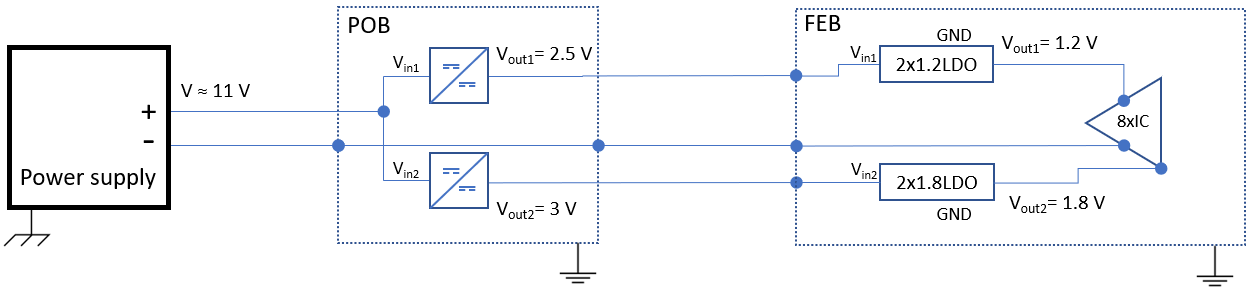
\includegraphics[width=1\columnwidth]{Chapter6/DCS/images/powering_diss_feb.png}
\caption{Schematics of the powering scheme of the \gls{FEB}. The focus was put on the elements that contribute the most to the overall power dissipation.}
\label{fig_power_scheme}
\end{figure}
% Please add the following required packages to your document preamble:
% \usepackage{multirow}
% \usepackage{graphicx}
\begin{table}[!h]
\centering
\caption{Power dissipation of the powering system in the function of the CSA registers values. Once the ASICs are configured, the digital line current remains constant. The SMX ASIC is denoted as Integrated Circuit (IC).}
\label{tab:distribution}
\resizebox{\textwidth}{!}{%
\begin{tabular}{cccccc}
\hline
\multirow{2}{*}{CSA register} & \multicolumn{5}{c}{Power dissipation {[}W{]}}                                                                                                                                                                             \\
                              & ASICs & 1.8\,V LDO regulator & 1.2\,V LDO regulator & \begin{tabular}[c]{@{}c@{}}DC/DC converter 3 V\\ distribution lines\end{tabular} & \begin{tabular}[c]{@{}c@{}}DC/DC converter 2.5 V\\ distribution lines\end{tabular} \\ \hline
15                            & 5.28  & 1.38                & 0.84                & 2.97                                                                             & 1.29                                                                               \\
63                            & 10.26 & 1.38                & 2.46                & 2.97                                                                             & 6.36                                                                               \\ \hline
\end{tabular}%
}
\end{table}

Figure~\ref{fig_power_CSA} illustrates the distribution of the power dissipation among the different elements of the powering system for different values of the \gls{CSA} current. While increasing the power consumption of the \glspl{ASIC}, there is also a  significant rise in the power dissipated by the DC/DC converters and distribution lines. %\newpage

\begin{figure}[h!]
\centering
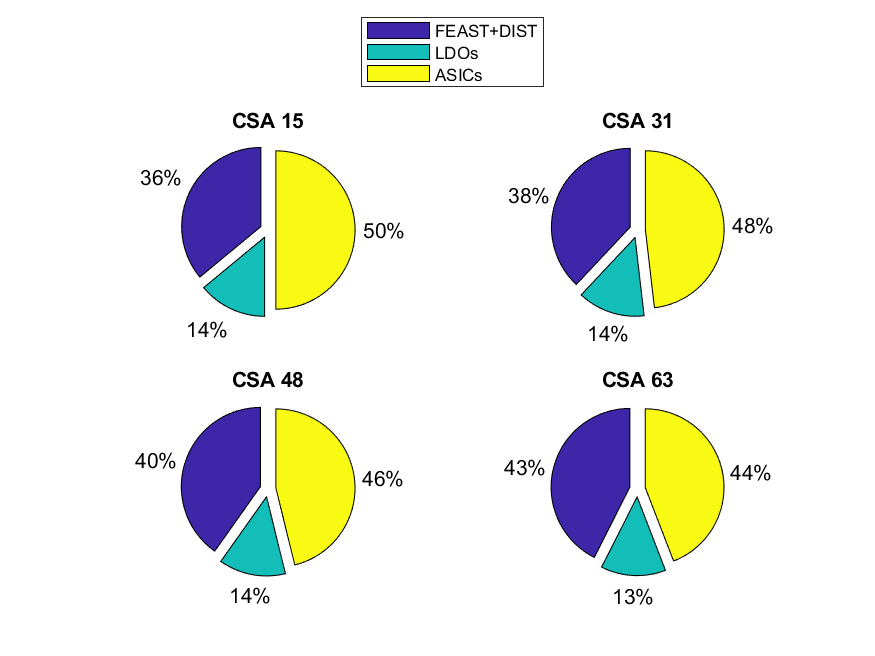
\includegraphics[width=0.6\columnwidth]{Chapter6/DCS/images/pie.png}
\caption{Power dissipation share of different elements of the power supply circuit as a function of the \gls{CSA} value.}
\label{fig_power_CSA}
\end{figure}

\newpage
Figure \ref{fig_power3} and \ref{fig_power4} show the current drawn by $4$ \glspl{FEB} of unit $1$ depending on the settings of the \gls{CSA}. It was determined that the \gls{CSA} value of $31$ should be the nominal value for the \gls{STS} modules. This value also ensures proper signal amplification, (\gls{CSA} value of $31$ corresponds to approximately $2$\,mA per analog channel). The \gls{CSA} value may vary from \gls{ASIC} to \gls{ASIC} to address the different requirements of the modules (depending for example on their noise levels). In principle, the \gls{ASIC} Analog Front End \gls{AFE} is powered by two power domains ($1.2$\,V - VDDM and $1.8$\,V - AVDD). By adjusting the \gls{CSA} registers settings, the VDDM domain is influenced. 
%\begin{figure}[h!]
%\centering
%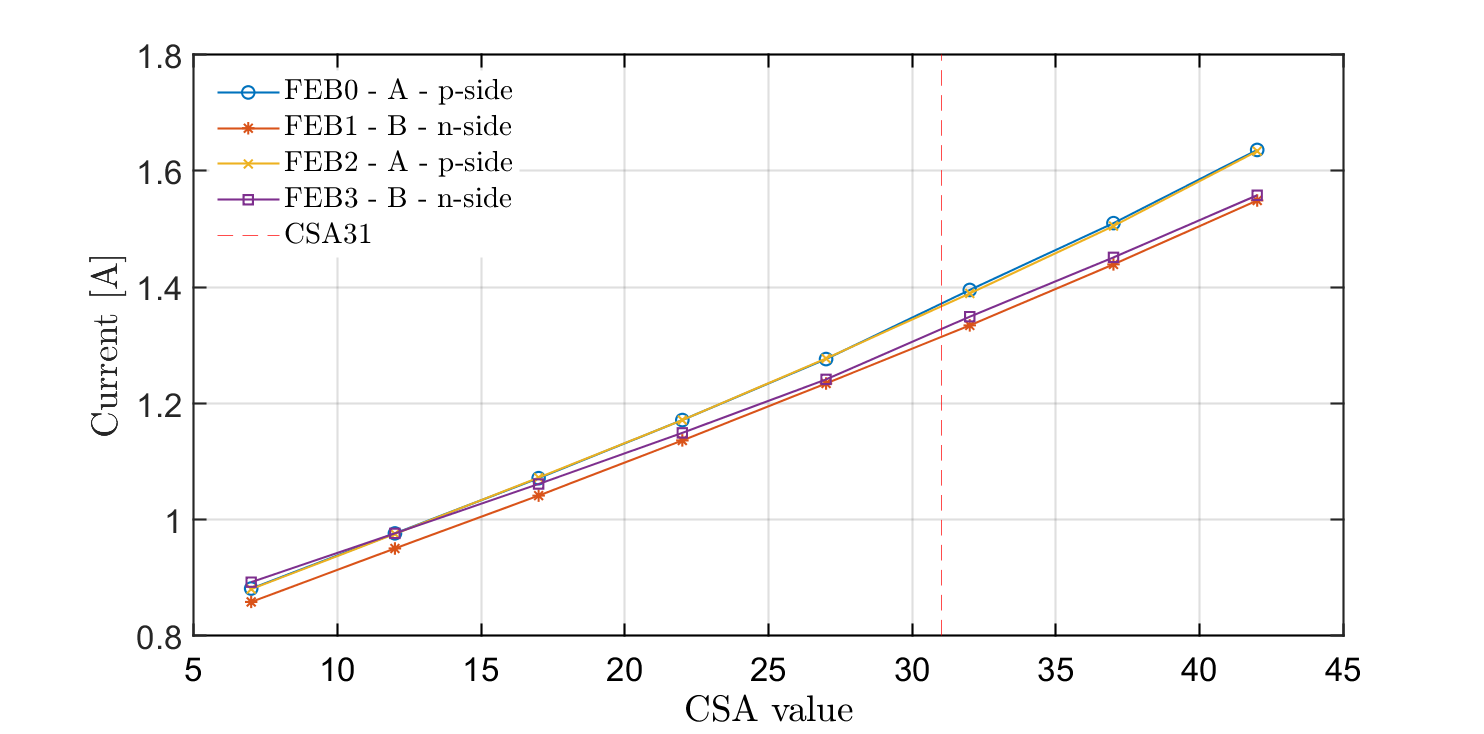
\includegraphics[width=0.45\columnwidth]{Chapter6/DCS/images/U0CSABIAS.png}
%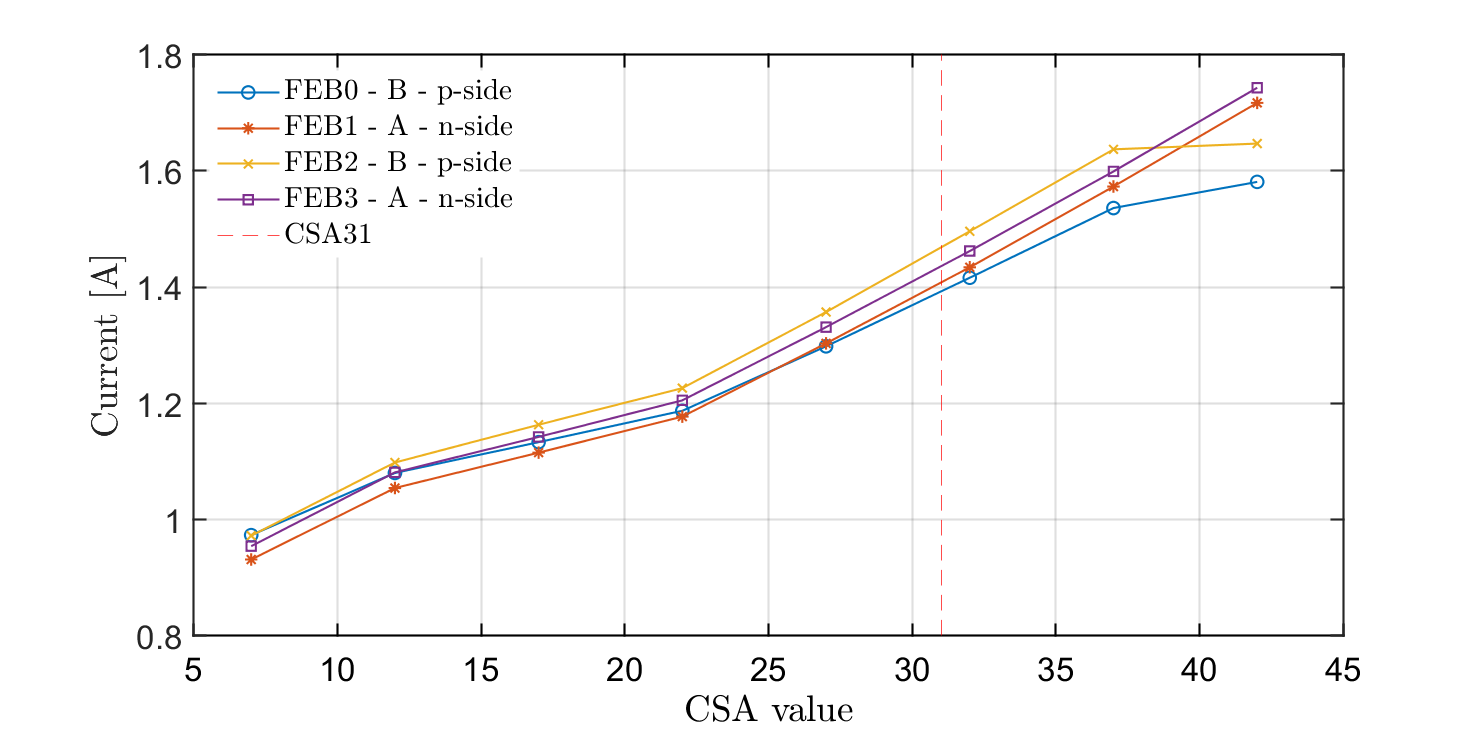
\includegraphics[width=0.45\columnwidth]{Chapter6/DCS/images/U1CSABIAS.png}
%\caption{CSA scan of the unit 0 (left) and 1 (right)}
%\label{fig_power1}
%\end{figure}
\begin{figure}[h!]
\centering
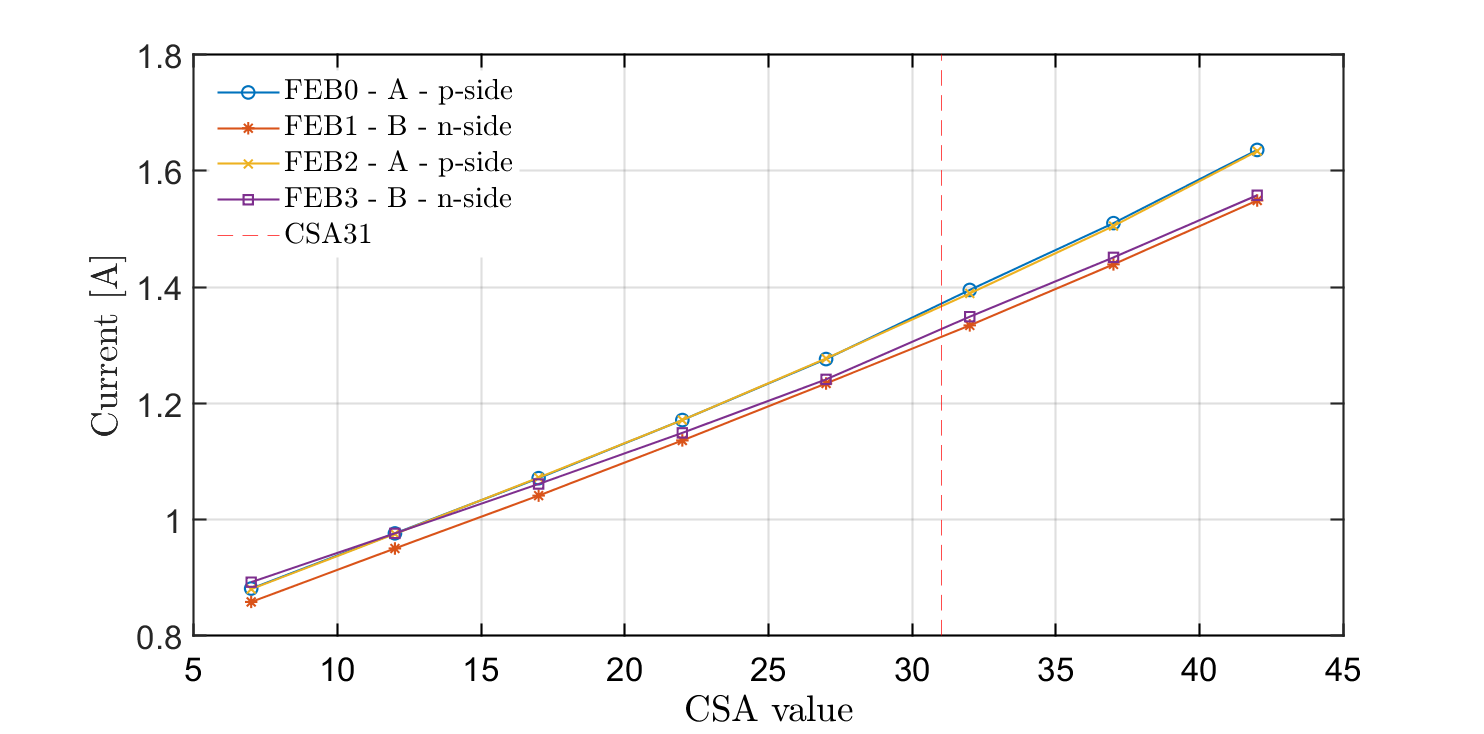
\includegraphics[width=0.9\columnwidth]{Chapter6/DCS/images/U0CSABIAS.png}
\caption{Low voltage \gls{FEB} current measured at the power supply in the function of CSA settings of unit 2. }
\label{fig_power3}
\end{figure}
\begin{figure}[h!]
\centering
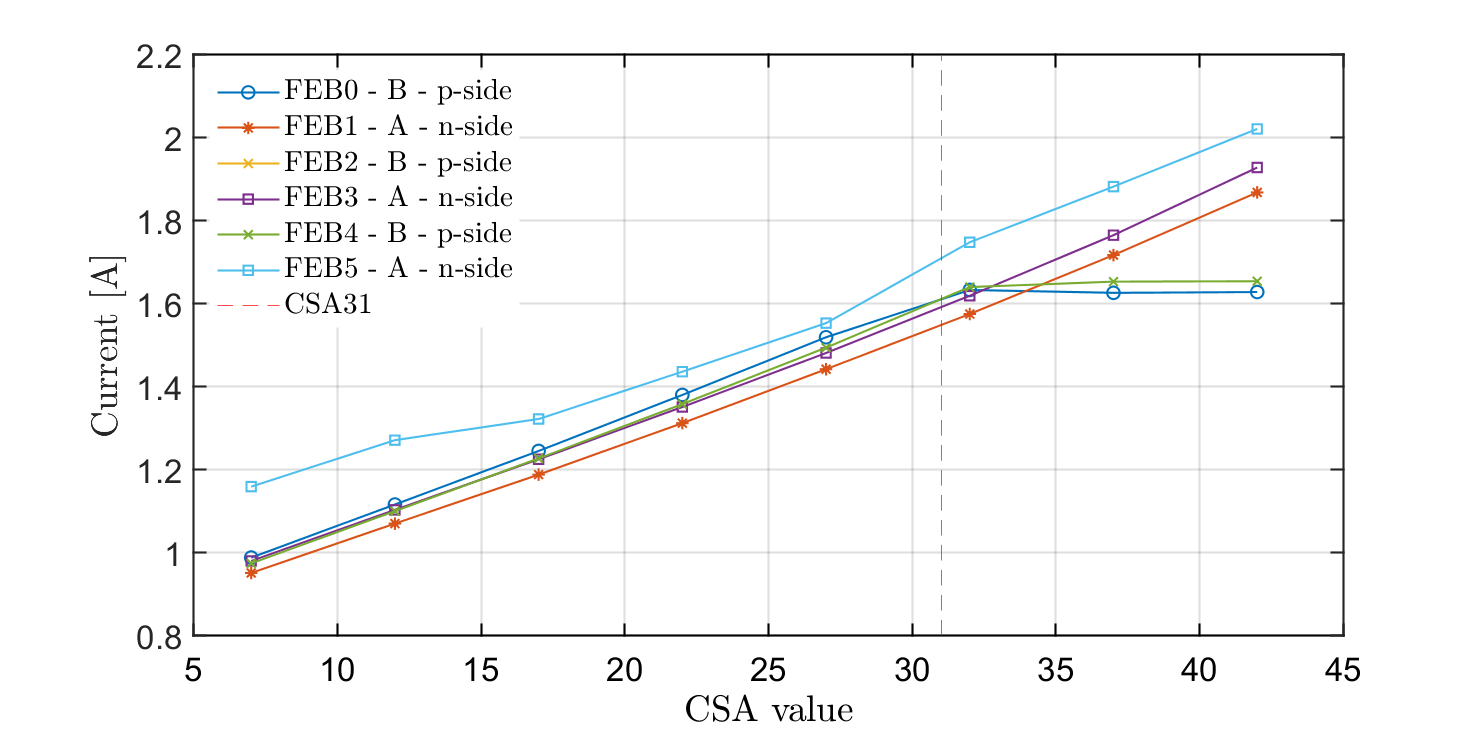
\includegraphics[width=0.9\columnwidth]{Chapter6/DCS/images/U3L0CSABIAS.png}
\caption{Low voltage \gls{FEB} current measured at the power supply in the function of CSA settings of the unit 3 ladder 0. FEB2 did not respond during the testing.}
\label{fig_power4}
\end{figure}

Similar measurements were also conducted for all the other detector modules (see Appendix~\ref{CSA}). The average values of the current for every unit are depicted in Figure \ref{fig_avg}. For the older modules, especially those powered by $2.4$\,V and $2.4$\,V DC/DC converters (unit $3$), the currents are significantly higher, reaching $1.6$\,A - $1.8$\,A at the \gls{CSA} $31$. The \gls{AFE} of the modules of unit $1$ are powered by the $1.8$\,V \gls{LDO} regulators with a diode, which causes a voltage drop of approximately $0.6$\,V. Nevertheless, this sub-optimal solution can be also seen via increased current and power dissipation of the unit $1$ modules. The modules current of units $0$ and $2$ are similar, as they use the same components, which are also considered the final ones for \gls{STS}.

%\newpage
\begin{figure}[h!]
\centering
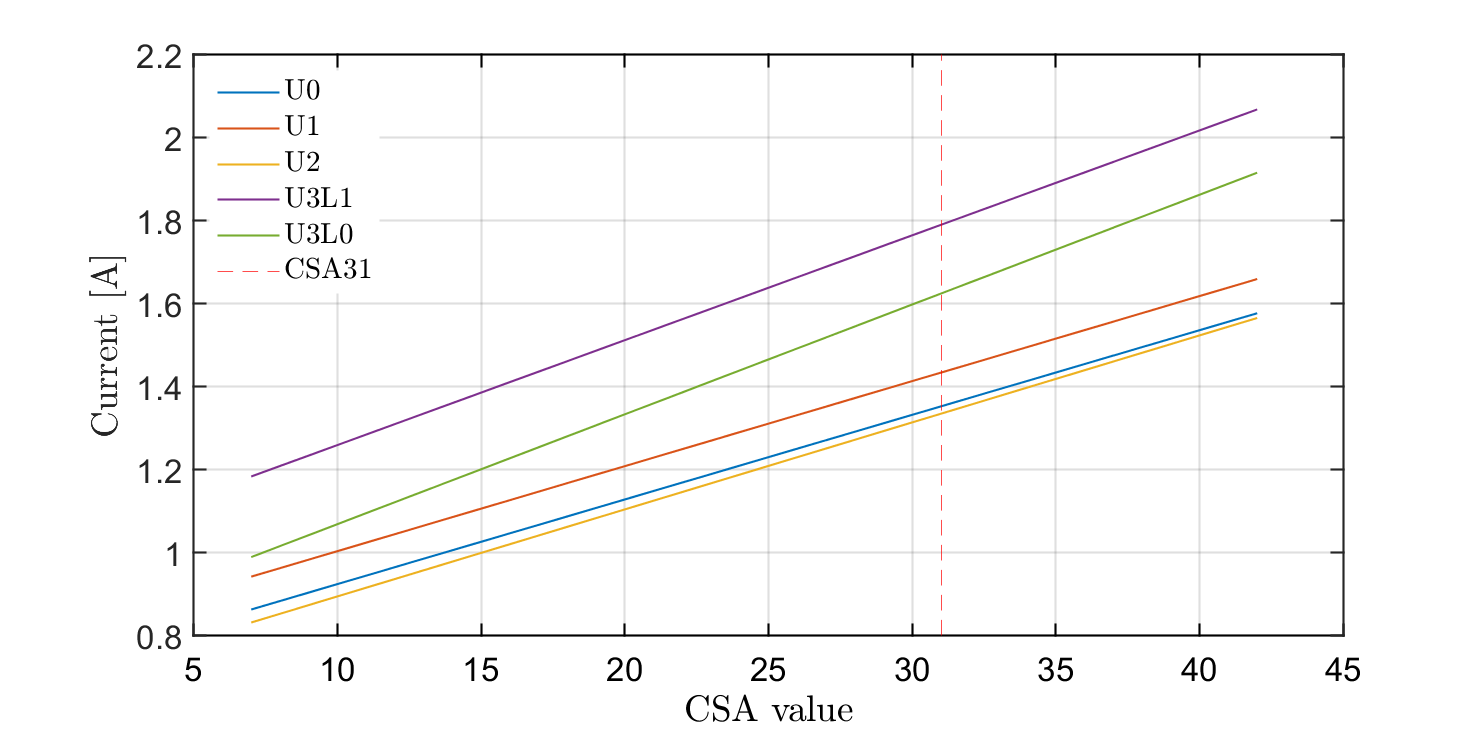
\includegraphics[width=0.9\columnwidth]{Chapter6/DCS/images/units.png}
\caption{Average current of each \gls{mSTS} unit.}
\label{fig_avg}
\end{figure}
\newpage
The \gls{mSTS} modules are powered in the constant voltage mode, which means that the output voltage is always $10.5$\,V. Knowing the currents at the power supply level, cable lengths, and voltage drops on subsequent components, it is possible to calculate the power dissipation. 
To estimate the power consumption based on the values from the module testing prior to the detector assembly. Average values of the currents are presented in Table \ref{tab:typical_cons}. By adding estimates related to the distribution lines and DC/DC converters from figure~\ref{fig_power_scheme} it is possible to compare these values with \gls{mSTS} results.
\begin{table}[!h]
\caption{Currents drawn by the analog front end and to the digital part depending on the set \gls{CSA} value.}
\centering
\begin{tabular}{lll}
\hline
CSA & Current digital {[}A{]} & Current \gls{AFE} {[}A{]} \\ \hline
15  & 1.9                 & 1.02                    \\
31  & 1.9                 & 2.05                    \\
48  & 1.9                 & 3.07                    \\
63  & 1.9                 & 4.10                    \\ \hline
\end{tabular}

\label{tab:typical_cons}
\end{table}

Figure \ref{fig_theor} shows the comparison of the power consumption of \gls{mSTS} units with the calculations based on the average current from the modules testing (depicted as FLA v2) and FEB currents measurement (denoted as FLA). 

\begin{figure}[h!]
\centering
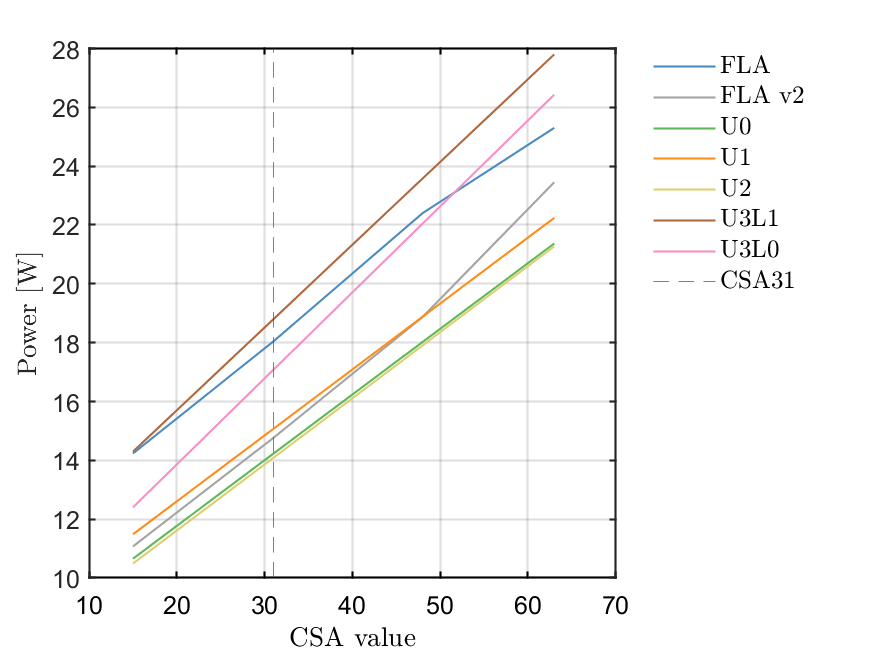
\includegraphics[width=0.95\columnwidth]{Chapter6/DCS/images/theor.png}
\caption{Average power dissipation of the units compared with predictions based on theoretical power dissipation in the components (depicted as FLA and FLA v2).} 
\label{fig_theor}
\end{figure}
The estimation based on the average current from the modules testing has the lowest power consumption values up to CSA of $48$. The values obtained from that estimation are close to those from units $0$ and $2$. These units are considered to be built from almost final components. Hence, the power consumption of these modules should serve as a reference for further calculations. Some parameters related to the voltage drop may change in \gls{STS}, mostly due to different powering lines lengths and diameters of the wires, as well as different connectors. 
\begin{table}[h!]
\caption{Total power consumption of the 876 modules of \gls{STS} based on the calculations from Figure~\ref{fig_theor}.}
\centering
\begin{tabular}{lll}
\hline
               & \gls{CSA} 31  & \gls{CSA} 48  \\ \hline
FLA estimation & 23.5 kW & 30.9 kW \\
Unit 3         & 30.2 kW & 35.7 kW \\
Unit 2         & 26.7 kW & 30.8 kW \\ \hline
\end{tabular}

\label{tab:power_cons}
\end{table}
The values stated in Table~\ref{tab:power_cons} can not be considered as a reference. The results provide an estimation of the power consumption and also show how the module assembly evolved. 
%\newpage
\subsection{Parameters monitoring and obtained data}
All the software and hardware components mentioned in the previous sections deliver essential information about the detector safety and operational state. Thanks to the ongoing ambient monitoring, many issues of the subsystem were discovered and addressed, e.g., not sufficient cooling. Figure \ref{fig_temp} shows the temperature trends obtained through \gls{DCS} during the 430 days of operation. The first temperature sensor (depicted in blue) was placed at the top of the \gls{mSTS} enclosure and the second one (depicted in orange) is located on the upper part of unit 2. Temperatures registered in \gls{mSTS} vary not only depending on the \gls{FEE} powering (peaks observed throughout the operation) but also on the temperature in the cave. The broader peak at the end of the studied period (red dashed line) is associated with the cooling unit failure. There are also a few periods, with the longest in December and January when the detector was not operated. 

\begin{figure}[!h]
\centering
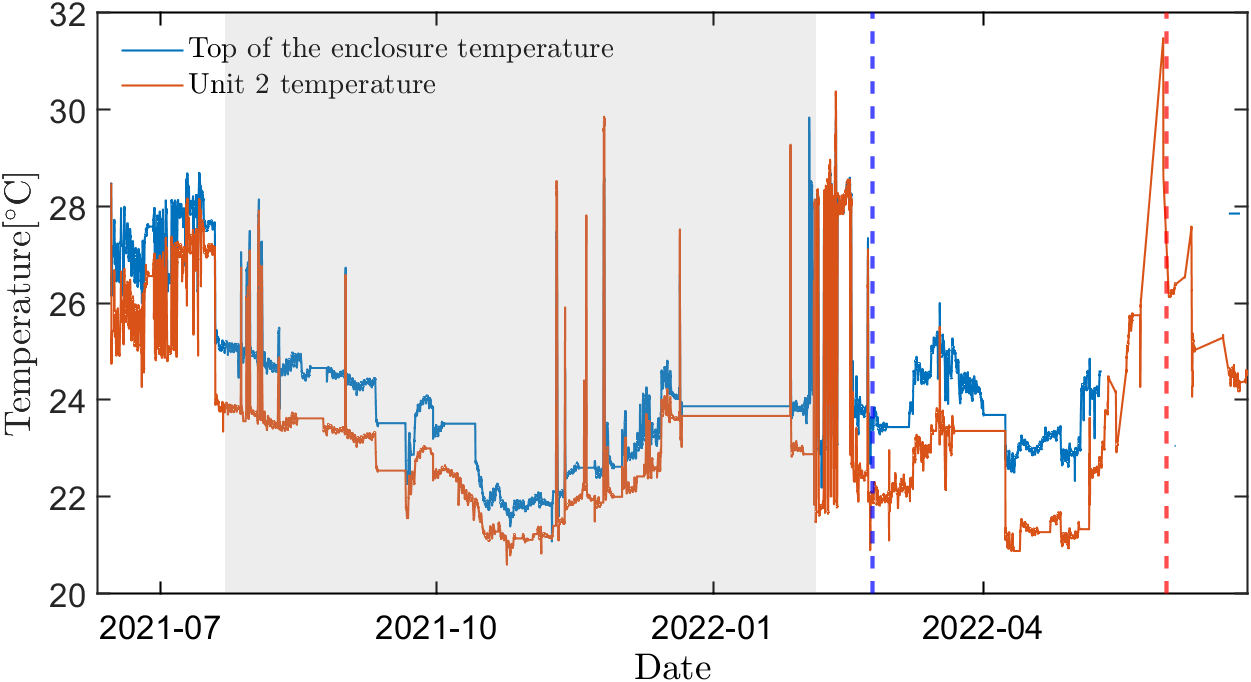
\includegraphics[width=0.9\columnwidth]{Chapter6/DCS/images/temp2.png}
\caption{Temperature monitoring in the \gls{mSTS} detector using PT100 sensors. The gray area refers to the period without any major data-taking activities.}
\label{fig_temp}
\end{figure}
\newpage
To ensure the safe operation of the system, it was also necessary to have information about the dew point. Water condensation on the parts of the \gls{FEE} could cause the electronics to fail. Figure \ref{fig_dew} depicts the trends in the dew point and temperature over the mentioned period. The coolant setpoint was always carefully adjusted depending on the situation in the experimental cave, and it varied between \SI{12}{\celsius} and \SI{17}{\celsius}.

\begin{figure}[!h]
\centering
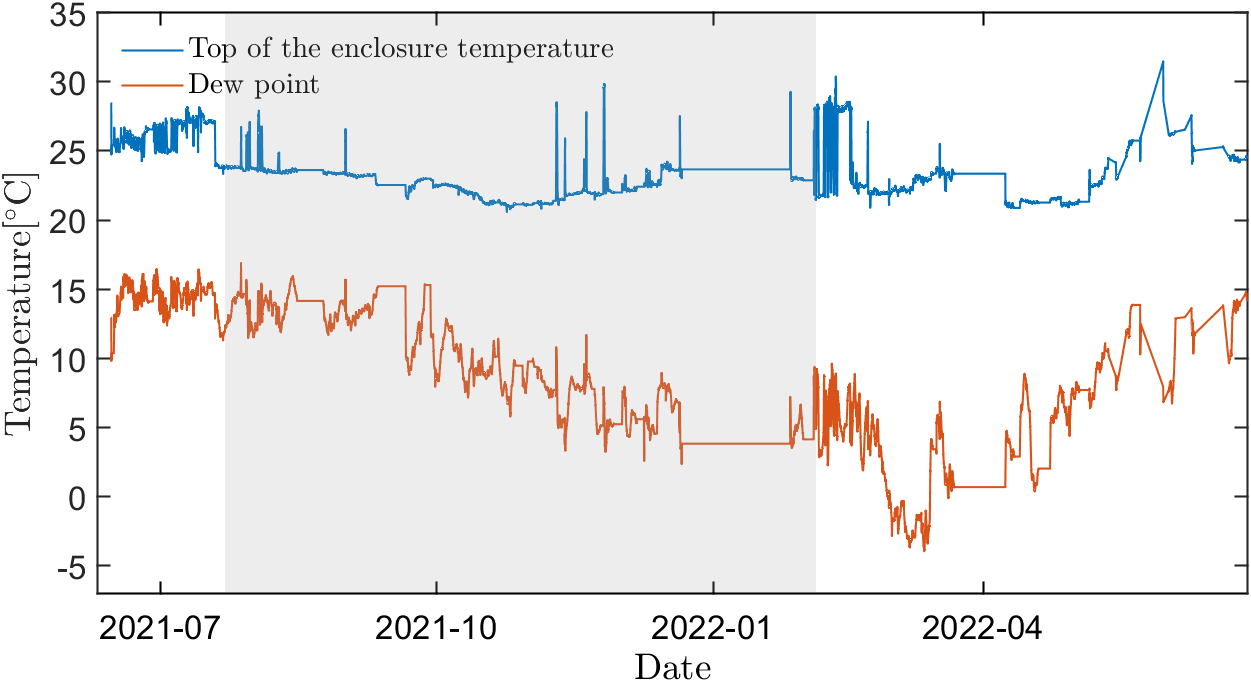
\includegraphics[width=0.9\columnwidth]{Chapter6/DCS/images/dew.png}
\caption{Temperature and dew point monitoring. Dew point calculations are based on the \gls{RH} and temperature measurement of the SHT85 sensor.}
\label{fig_dew}
\end{figure}


Temperature sensors (PT100) are also used to monitor the temperature on the powering boards. A comparison of the temperatures on the \gls{POB} of units $1$, $2$, and between two \glspl{POB} of unit 3 are presented in Figure~\ref{fig_POB1}. The temperature measured in unit $3$, especially at the beginning of the operation (depicted with the red rectangle), was much higher than those measured in units $0$ and $1$. This effect is associated with insufficient cooling which was resolved at the beginning of $2022$. At the right end of the plot, cooling unit failure is also visible.
\begin{figure}[!h]
\centering
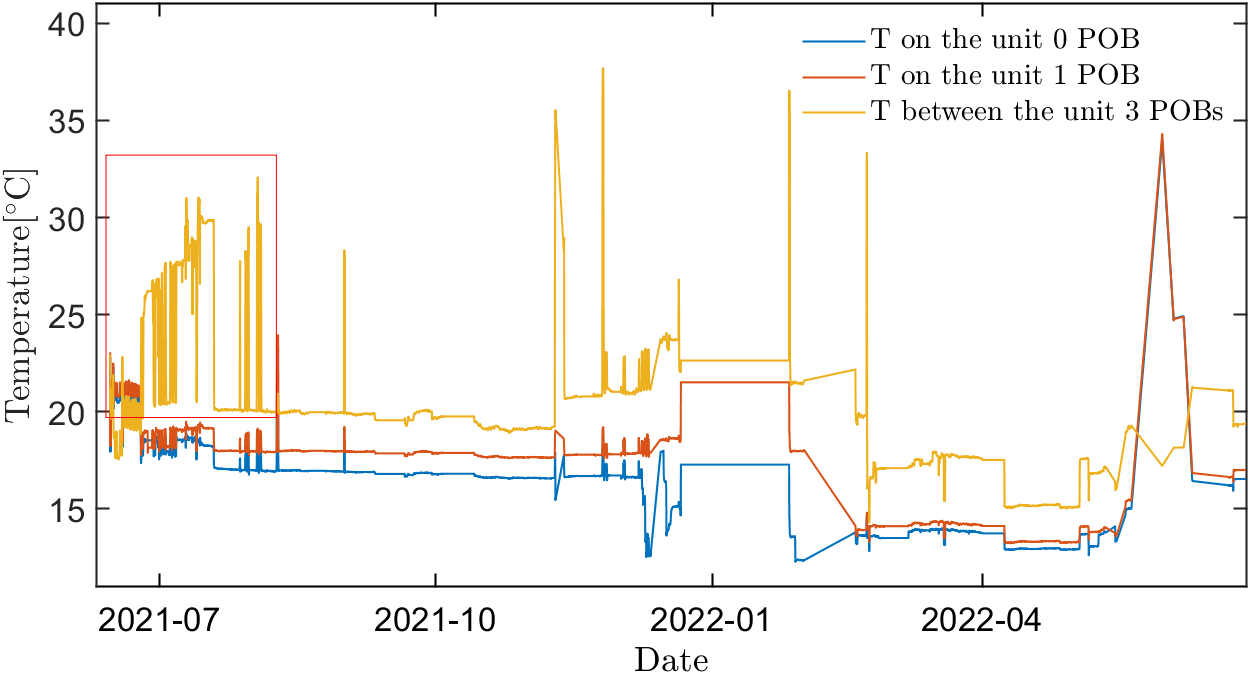
\includegraphics[width=0.9\columnwidth]{Chapter6/DCS/images/POB1.png}
\caption{Temperature monitoring on the \glspl{POB} enclosure using the PT100 sensors.}
\label{fig_POB1}
\end{figure}

Additionally, the temperature on the \gls{ROB} and \gls{FEB} was monitored, as depicted in Figure~\ref{fig_robvsfeb}. Interestingly, the temperature on the \gls{ROB} is higher than the temperature on the \gls{FEB} box on unit $2$. Unit $2$ features $2$ modules, $4 $\gls{FEB}s (+ pulser board) in the \gls{FEB} box (each drawing about $1.6$\,A at constant $10.5$\,V), in comparison to the \gls{ROB} which is powered with $7$\,V and consumes about $0.8$\,A. This is, most likely, related to the better contact of the \gls{FEB} box to the cooling plate.

\begin{figure}[!h]
\centering
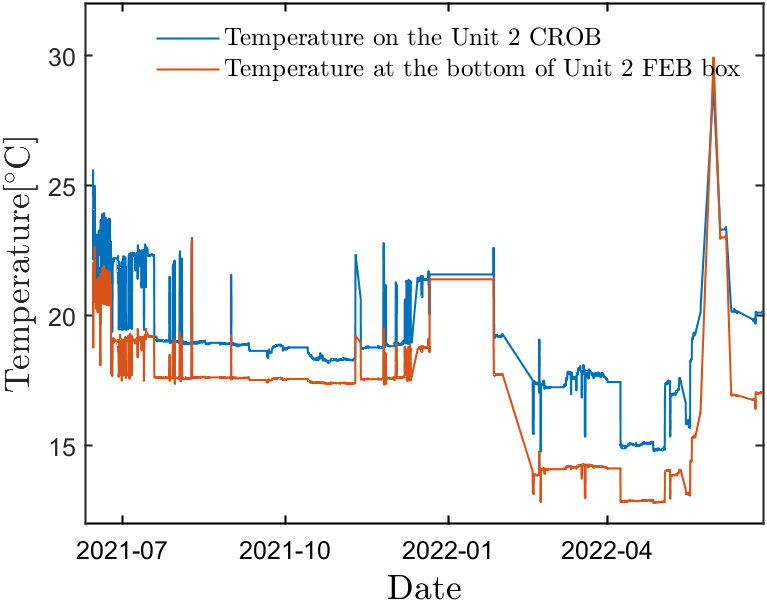
\includegraphics[width=0.9\columnwidth]{Chapter6/DCS/images/ROBvsFEB.png}
\caption{Temperature on the \gls{ROB}, and underneath the\gls{FEB} box using the PT100 sensors}
\label{fig_robvsfeb}
\end{figure}

\newpage

\subsection{Monitoring of the leakage current}

Information about the temperatures serves not only to ensure detector safety but also to properly understand the behavior of the silicon sensors. Knowing the temperature trends over the irradiation period, it is possible to normalize the leakage current from different points to a certain reference value, e.g., \SI{20}{\celsius}. Firstly, if the exact temperature characteristic of the sensors is now known, it is necessary to rely on a temperature sensor placed close to the semiconductor. In the \gls{mSTS} several temperature  sensors are measuring ambient conditions, an overview can be seen in figure \ref{fig_temperatures}. The temperature inside the box is significantly lower, which indicates properly working cooling. Higher temperatures are also seen on the top of the detector, where the excess heat is not evacuated. 

\begin{figure}[!h]
\centering
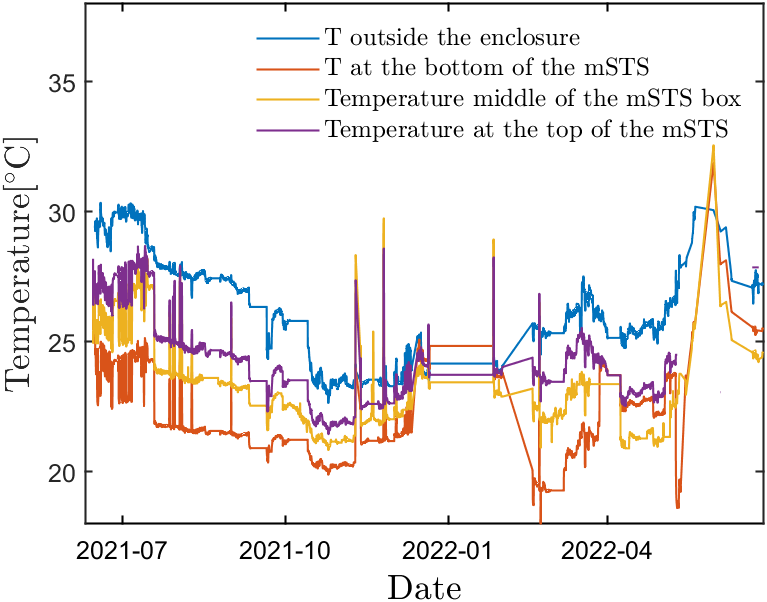
\includegraphics[width=0.9\columnwidth]{Chapter6/DCS/images/rates/tempmSTS.png}
\caption{Comparison of the temperatures inside \gls{mSTS} with the temperature in the experimental cave.}
\label{fig_temperatures}
\end{figure}

As the silicon sensors are symmetrically biased, the nominal operating voltage was chosen to be $\pm75$\,V (to assure full depletion of the non-irradiated silicon sensors). The reverse polarity also implies negative current values. In most of the plots, the leakage current of only one side of the silicon sensors will be shown. The other side of the sensor is characterized by the same trends but with opposite sign.

%\newpage
\begin{figure}[!h]
\centering
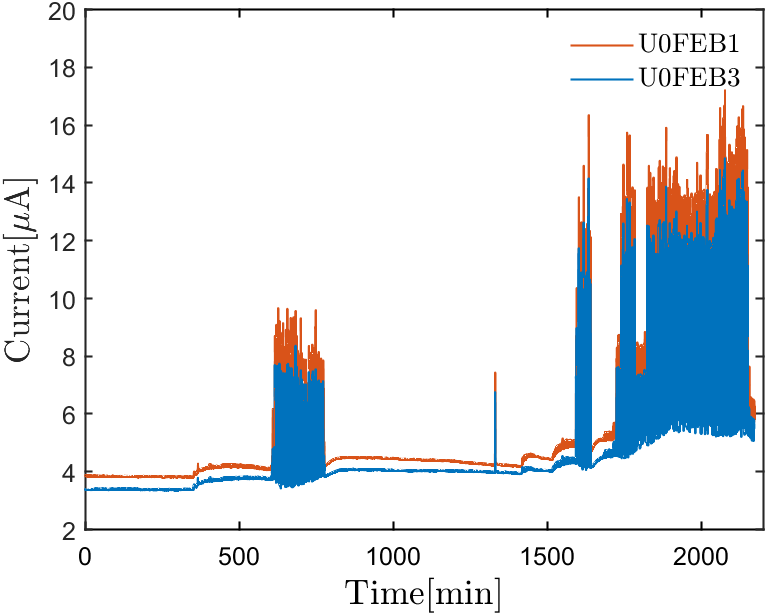
\includegraphics[width=0.45\columnwidth]{Chapter6/DCS/images/uranium/U0.png}
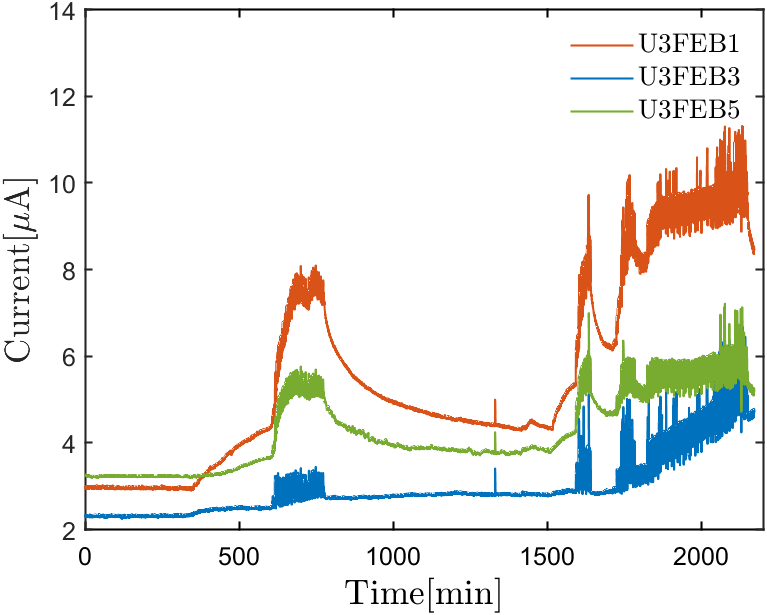
\includegraphics[width=0.45\columnwidth]{Chapter6/DCS/images/uranium/U3.png}
\caption{Leakage current of the silicon sensors in modules of units $0$ and $3$ during collisions of U ions with the Au target of different thicknesses.}
\label{fig_msts_LC}
\end{figure}

The leakage current changes of the \gls{STS} silicon sensors during data-taking can be seen in figure~\ref{fig_msts_LC}. Due to radiation-induced surface and bulk damage, the leakage current  increased with the increasing total fluence (as foreseen in the Hamburg Model). In order to properly compare the leakage current before and after the irradiation, it is necessary to have the same ambient conditions or to measure the temperature and then normalize the current to \SI{20}{\celsius}. Apart from the constant rise of the leakage current during the data-taking, two particular parts of the plot can be distinguished. The first one just after $600$\,min, when increased beam intensity (about $10^{8}$\,ions/spill) caused the spill structure to appear. A similar trend can also be observed from around 1600 min. The sensors of different units behave slightly differently, depending on their position relative to the beam, sensor size, or possible differences in the assembly procedure.


\begin{figure}[!h]
\centering
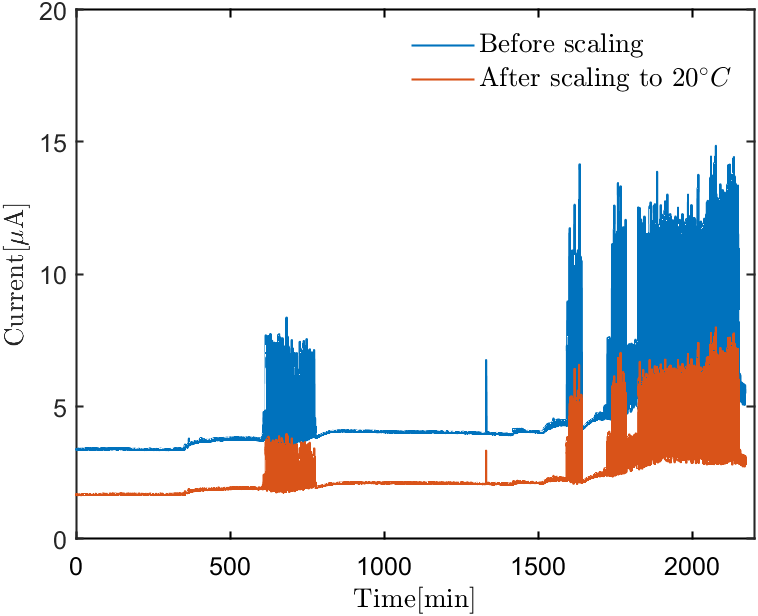
\includegraphics[width=0.45\columnwidth]{Chapter6/DCS/images/uranium/current_U_highintensity.png}
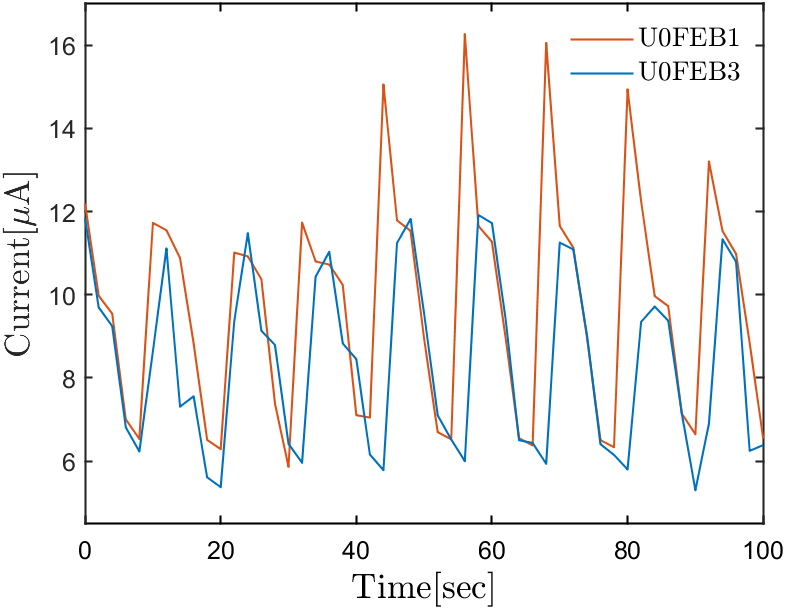
\includegraphics[width=0.47\columnwidth]{Chapter6/DCS/images/uranium/U3L1_spill.png}
\caption{Unit $0$ \gls{FEB} $3$- normalization of the current (left) and zoomed-in view of the spill structure seen by the silicon sensors (spill of $10$\,s length).}
\label{fig_sensors_spill}
\end{figure}

An example of the normalization of the unit $0$ sensors is depicted in Figure~\ref{fig_sensors_spill}. A more detailed view of the spill structure is shown on the right plot. It can be clearly seen, that the reaction products traversing the silicons cause a significant leakage current increase of about \SI{10}{\micro A} (for the highest beam intensities - $10^{9}$ ions/s). Comparison of the average leakage current from two units after normalization to $20\,^{\circ}$C is shown in Figure~\ref{fig_leak}. Throughout the year $2021$, only a few beam time campaigns took place. The increase in the leakage current due to radiation-induced damage is negligible. On the other hand, during the beam campaigns of $2022$, the effect of radiation can be clearly seen. The leakage current value obtained for module $0$ of unit $3$ differs from the performance of other modules, indicating an electrical problem.

\begin{figure}[!h]
\centering
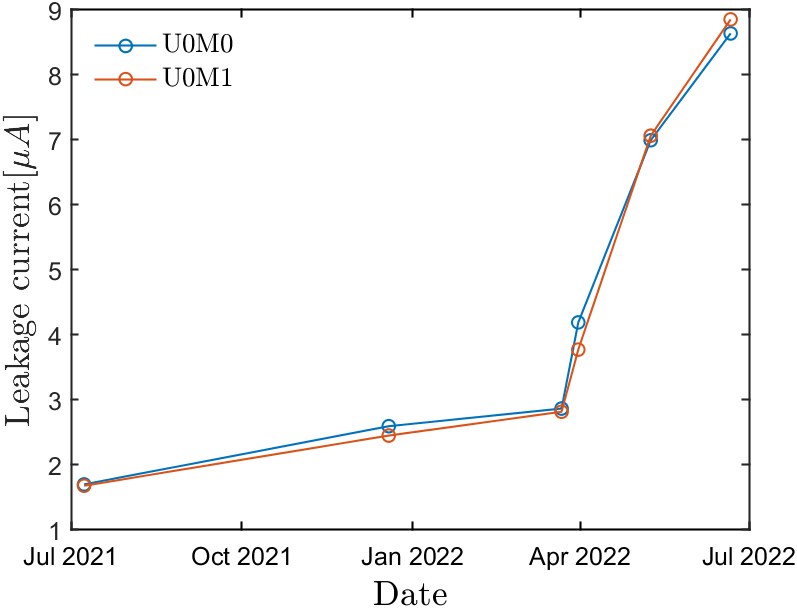
\includegraphics[width=0.48\columnwidth]{Chapter6/DCS/images/sensors/U0_leakage.png}
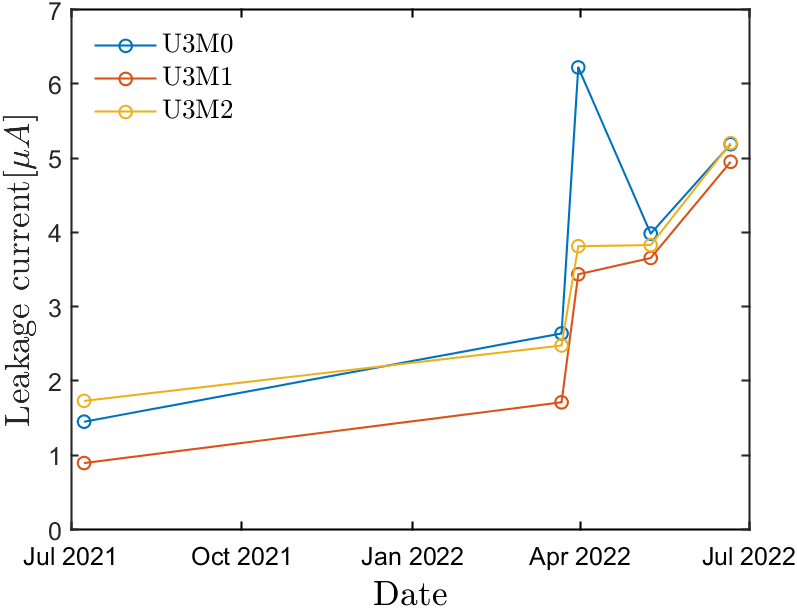
\includegraphics[width=0.48\columnwidth]{Chapter6/DCS/images/sensors/U3_leakage.png}
\caption{Average leakage current evolution of the \gls{mSTS} sensors over the $430$ days of operation. }
\label{fig_leak}
\end{figure}

The quantitative current changes over the \gls{mCBM} campaign are shown in Table~\ref{tab:msts_final_fluence}. To better understand the overall results, it is important to take a look at the position of the silicon sensors with respect to the beam (see~figure~\ref{fig_sensors_scheme}). The sensors located closer to the collision point (from unit $0$) are more irradiated than sensors from units $2$ and $3$. Furthermore, the results obtained from unit $3$ are inconsistent throughout the experiment, which means that those modules seem to experience electrical problems (e.g., short circuits). By applying the formulas introduced in Chapter~\ref{silicon_damage}, it is possible to estimate the fluence accumulated by the sensors based on the leakage currents differences (Table~\ref{tab:msts_final_fluence}).
The major uncertainty is connected to the damage coefficient ($\alpha$). The $\alpha$ of $5,53\times 10^{-17}\,\mathrm{A/cm}$ was chosen based on the analysis prepared by~\cite{Larionov:2016eoz}. 

\begin{table}[!h]
\caption{Leakage current differences and corresponding fluence estimations based on the Hamburg model for all the \gls{mSTS} modules.}
\centering
\begin{tabular}{lcc}
\hline
\multicolumn{1}{c}{Module} & \begin{tabular}[c]{@{}c@{}}Current \\ difference {[}uA{]}\end{tabular} & Fluence {[}$\mathrm{n/cm_{2}}${]} \\ \hline
U3L1M0                     & 16.2                                                                  & $2.5\times10^{11}$          \\
U3L1M1                     & 7.6                                                                    & $5.8\times10^{10}$          \\ \hline
U3L0M0                     & 3.7                                                                    & $5.7\times10^{10}$          \\
U3L0M1                     & 4.1                                                                    & $6.2\times10^{10}$          \\
U3L0M2                     & 3.5                                                                    & $5.3\times10^{10}$          \\ \hline
U2M0                       & 3.6                                                                    & $5.5\times10^{10}$          \\
U2M1                       & 6.3                                                                    & $4.8\times10^{10}$          \\ \hline
U1M0                       & 6.4                                                                    & $9.8\times10^{10}$          \\
U1M1                       & 6                                                                      & $9.1\times10^{10}$          \\ \hline
U0M0                       & 6.9                                                                    & $1.1\times10^{11}$          \\
U0M1                       & 7.2                                                                    & $1.1\times10^{11}$ \\ \hline       
\end{tabular}
\label{tab:msts_final_fluence}
\end{table}

\begin{figure}[!h]
\centering
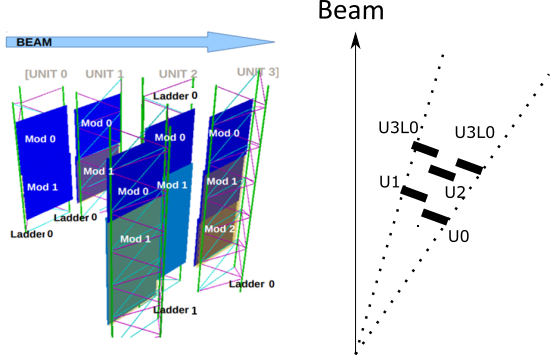
\includegraphics[width=0.65\columnwidth]{Chapter6/DCS/images/msts_sensors_scheme2.png}
\caption{Schematic view of the \gls{mSTS} sensor position with respect to the beam}
\label{fig_sensors_scheme}
\end{figure}
\newpage
\subsection{Current-voltage characteristic of chosen modules}
The dependence of current on the biasing voltage provides (IV) crucial information about the detector performance (see section \ref{sensors}):
\begin{itemize}
    \item Shot noise, closely related to the leakage current, which increases with the fluence
    \item Type inversion
    \item Annealing, and reverse annealing processes
\end{itemize}
Figure \ref{fig_IV} shows IV curves of two selected modules from two different units ($1$ and $3$) measured before assembly and at different moments of the module operation in the \gls{mSTS}.
\begin{figure}[!h]
\centering
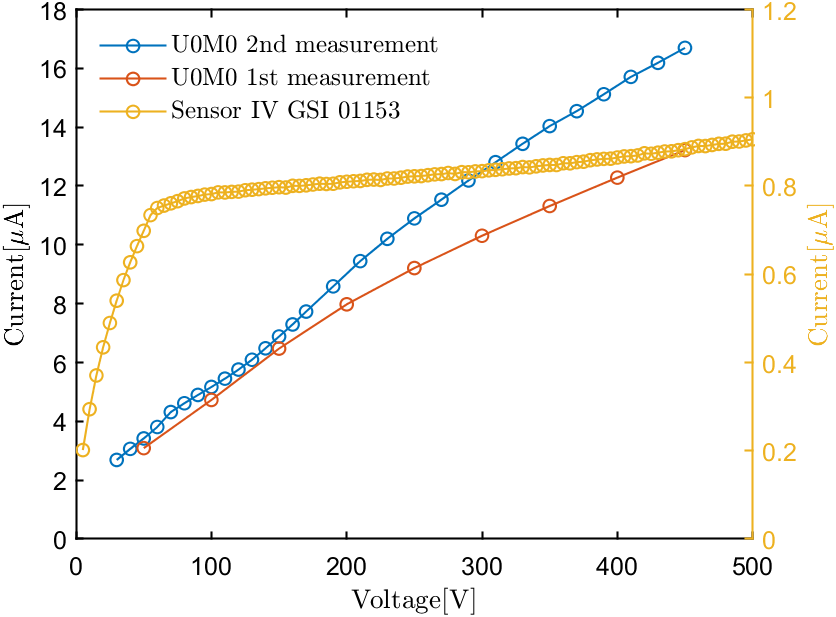
\includegraphics[width=0.48\columnwidth]{Chapter6/DCS/images/IV/U0FEB1.png}
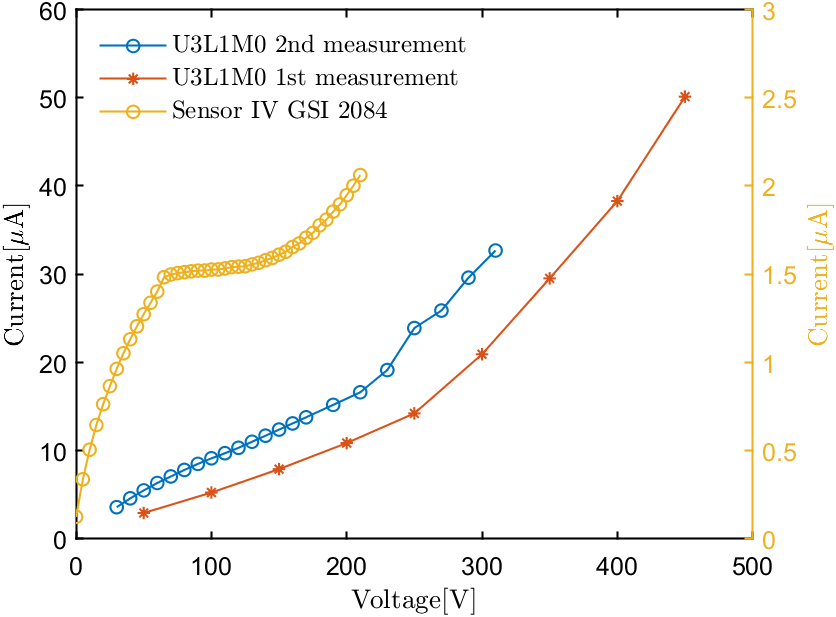
\includegraphics[width=0.48\columnwidth]{Chapter6/DCS/images/IV/U3L1FEB1.png}
\caption{IV curves for two modules from different \gls{mSTS} units (Left: module $0$ of unit $0$, right: module $0$ of ladder $1$ of unit $3$). Silicon sensors were tested in the clean laboratory (yellow curve), then subsequently after the first beam time (with U ion beam) and at the end of the test period in June $2022$ (second measurement).}
\label{fig_IV}
\end{figure}
Leakage current measurements are scaled down to $\SI{20}{\celsius}$ but the relative humidity was different for each measurement. The IV measured during the QA procedure before the assembly of the module is depicted in yellow and shows a typical behavior of a reverse-biased silicon diode with a full depletion reached around $60$-$70$\,V. The two other IV measurements for each module took place after assembly in \gls{mSTS}, the beam campaign with the U beam, and at the end of data-taking for $2022$. The linear behavior of the sensors can be seen after the module assembly, measuring with an external high-voltage filter in a floating scheme and low-voltage powering lines. Even though it is difficult to distinguish the point of full depletion, the current was still in the expected range. The unit 3 sensor shows a breakdown at a similar biasing voltage for all three measurements.


Figure~\ref{fig_IV_good} shows the IV measurement of a module assembled similarly to the ones used in the \gls{mSTS} detector. This module was tested without additional \gls{HV} filter, \gls{LV} connection, and the Keithley~\cite{Keithley} power supply instead of ISEG \gls{HV} module. The \gls{HV} filter was integrated into the new version of the \gls{FEB} (FEB8-3).


Linear behavior of the current-voltage characteristics from Figure~\ref{fig_IV} indicates a resistive element added to the circuitry, which is related to the \gls{LV} power supply. The system is operated in the floating ground scheme. The LV power supplies in reality are not completely floating, but they have a floating regulator which starts conducing current above a certain threshold voltage. Since the system is highly integrated and compact, it’s not always possible to remove the LV connection to the module, hence the unwanted resistive part persists. Therefore, when measuring the IV we do not only observe the typical IV curve for the silicon sensor in reverse mode but also the resistive behavior coming from the LV power supply.
\begin{figure}[!h]
\centering
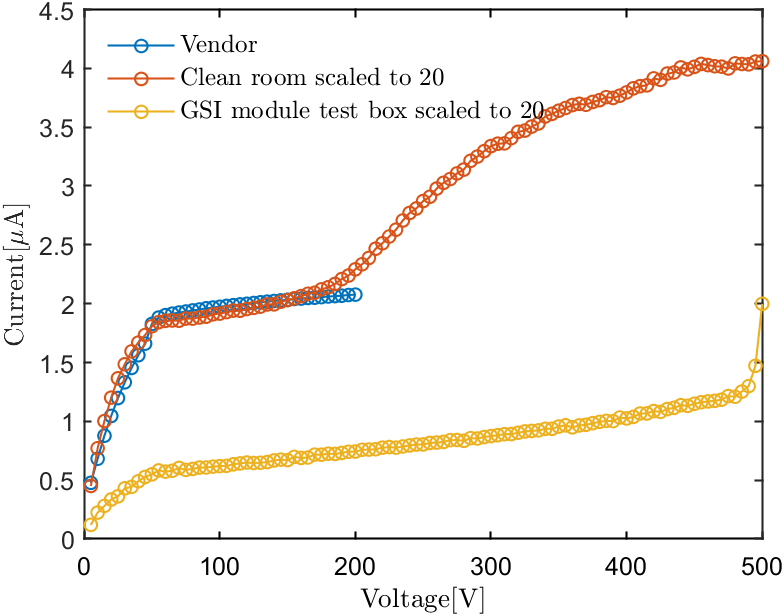
\includegraphics[width=0.5\columnwidth]{Chapter6/DCS/images/IV/30304Whole.png}
\caption{IV curves of another silicon sensor measured by the vendor before shipping, before the assembly, and then after it.} 
\label{fig_IV_good}
\end{figure}
\subsection{Data rates and leakage current}
Data rates from subsystems contain essential information about the detector performance. Figure~\ref{fig_data_rates_Ag} shows an example of the \gls{mCBM} Au+Au system ($T= 1\,\mathrm{AGeV}$) and later with Ni+Ni system, due to reaching the maximum data transfer (without the \gls{mSTS} detector). Data rates are clearly correlated with the beam intensity. Regardless of the beam intensities, \gls{mSTS} (with the chosen settings) is responsible for more than half of the total data. During the beam intensities of $10^{8}$ ions/s, \gls{mSTS} data rate was around 500 MB/s, and with the maximum beam intensities, it scaled up $2000$\,MB/s, reaching the limits of the data transmission for a \gls{FEB} $8$ with $2$ uplinks per \gls{ASIC}. 
\begin{figure}[H]
\centering
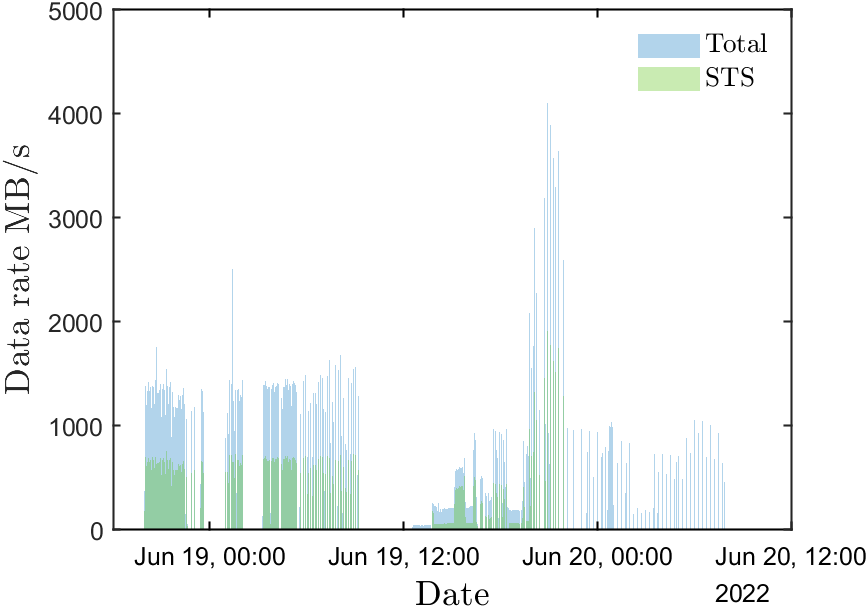
\includegraphics[width=0.6\columnwidth]{Chapter6/DCS/images/rates/Ag_total.png}
\caption{Data rates of all the \gls{mSTS} units in comparison to the overall data rate of all subsystems during data-taking.}
\label{fig_data_rates_Ag}
\end{figure}
There is a direct correlation of the leakage current increment with the beam intensity, which also determines the \gls{mSTS} data rate (see Figure~\ref{fig_Data}). This correlation gives more insight into the operation and state of the silicon sensors.
\begin{figure}[!h]
\centering
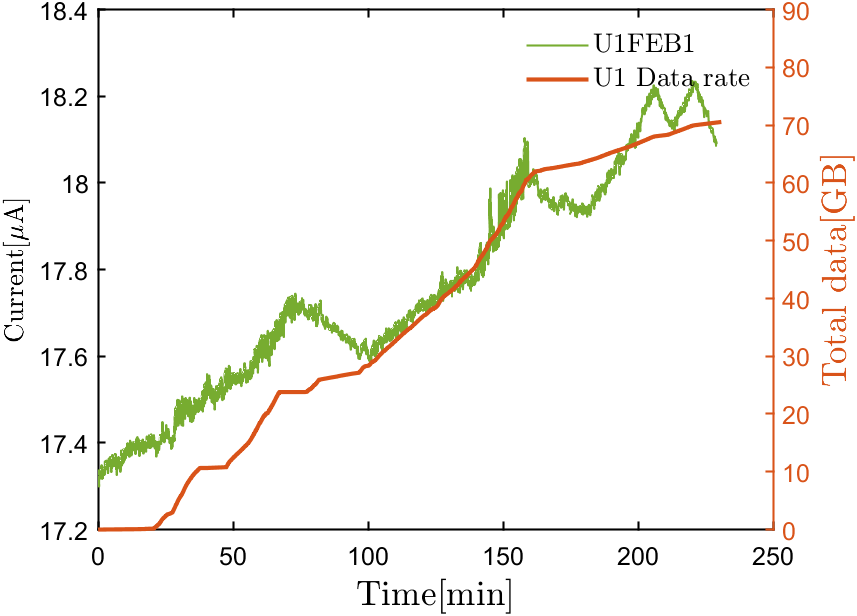
\includegraphics[width=0.48\columnwidth]{Chapter6/DCS/images/U1_data_rate.png}
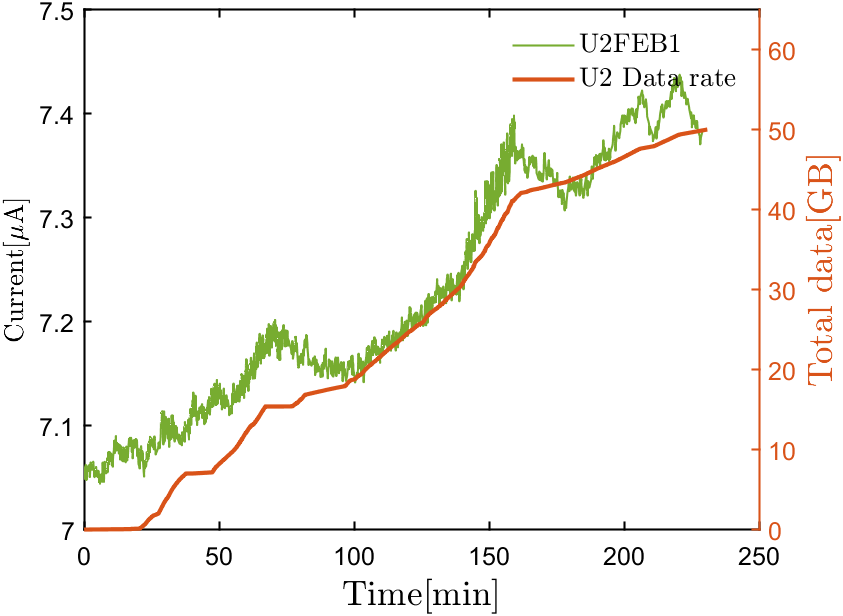
\includegraphics[width=0.48\columnwidth]{Chapter6/DCS/images/U2_data_rate.png}
\caption{Leakage current evolution of the \gls{mSTS} silicon sensors and respective integrated data rate.}
\label{fig_Data}
\end{figure}

\section{Conclusions}

The successful operation of the \gls{mSTS}, including the \gls{DCS} and \gls{DAQ} chain, set an important milestone toward the completion of the \gls{STS} project. The first extensive and successful data-taking activities with two tracking stations concluded the commissioning of the \gls{mSTS} detector. The prototyping of the \gls{DCS} supervisory layer of \gls{mSTS} took place, and it was successfully implemented, proving that the concept was extremely flexible and useful, not only for large detectors, and accelerator setups but also for smaller experiments. After almost two years of operation, container based system was found to be a reliable, easily maintainable solution. Yet, for the final system, several additional applications are needed. The \gls{STS} detector will be much more complex and challenging when it comes to configuration and operation. For the final setup, it will be extremely important to have both hardware and software interlocking to ensure the machine safety.

\gls{mSTS} did not publish its overall status to any external software agent. Due to that reason, some information like \gls{ASIC} internal temperature or VDDM were only accessible via the data acquisition chain (\gls{DCA}-\gls{CRI}). In the future, each subsystem will have an assigned Subsystem Control Agent (\gls{SCA}) to tackle control of the readout chain and the \gls{DCS}. 


Temperature sensors located inside the \gls{mSTS} and information about the current drawn by the sensors indicate the silicon sensors state. The sensors may degrade over time due to radiation-induced damage,  which leads i.a. to the leakage current increase, type inversion, etc. Those effects can be partially studied through the \gls{DCS} and the control strategy adopted respectively to the results.

Figure \ref{fig_dcs_results} shows how the \gls{DCS} performed during about $2$ years of operation. Due to the radiation-induced soft errors in the controllers of the cooling units, there were several occasions that the operation of the \gls{STS} had to be halted. Usually, such an interruption in the operation was automatically triggered by the \gls{FSM}. Listed errors might also include the intervention in the system. In that case, the error related to the cooling system was logged, but the FSM might have been off.
\begin{figure}[!h]
\centering
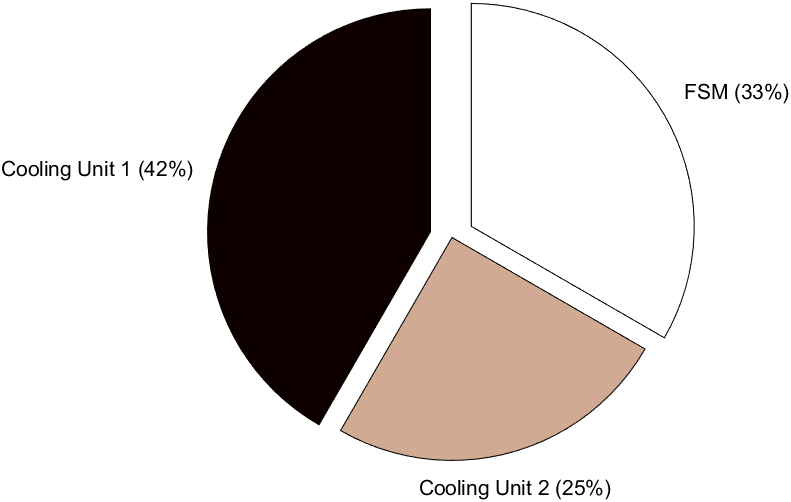
\includegraphics[width=0.55\columnwidth]{Chapter6/DCS/images/DCSpie.png}
\caption{Results from the operation.}
\label{fig_dcs_results}
\end{figure}

%The next chapter gives a more detailed explanation of the next steps which should follow the successful implementation of the containerized \gls{DCS}. In addition to that, the missing pieces of the system are also discussed.